\section*{Exercice 131 -- Correcteurs}
\setcounter{exo}{0}
%CCS PSI 2009
Les paliers magnétiques sont conçus, réalisés et montés par la société S2M.
Deux paliers radiaux assurent le guidage radial de l'arbre. Un troisième
palier assure le guidage axial. Un moteur électrique, placé entre les deux
paliers radiaux, entraîne le rotor en rotation. Le guidage magnétique consiste à exercer des efforts sur l'arbre en générant un
champ magnétique. Il n'y a donc aucun contact entre le bâti et l'arbre.

\begin{center}
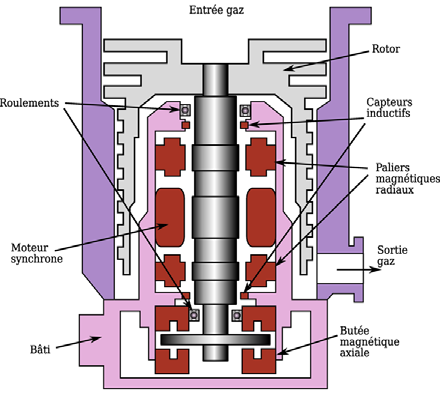
\includegraphics[width=.8\linewidth]{fig_05}
\end{center}


\begin{obj}
Déterminer la structure et les paramètres du correcteur à utiliser pour satisfaire les performances exigées.
\end{obj}


\begin{center}
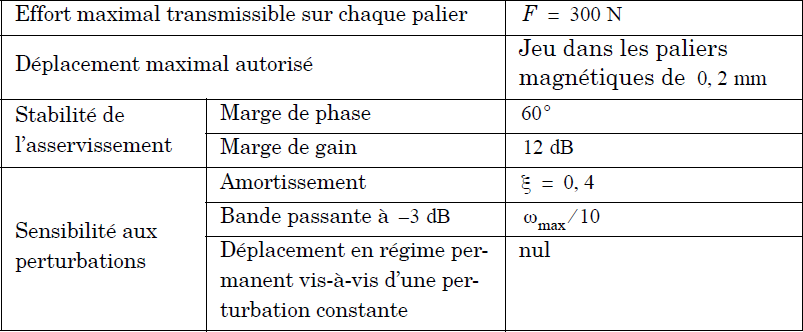
\includegraphics[width=\linewidth]{fig_04}
\end{center}


Afin de satisfaire les critères du cahier des charges, on envisage d'asservir un
palier magnétique par un premier bouclage de stabilisation (retour $K_D p+K_P$).
Un second retour unitaire associé à un correcteur $C(p)$ assure la régulation en
position du palier. On utilisera par la suite les
paramètres suivants : $K_e=\SI{5000}{V.m^{-1}}$, $K_0=\SI{190}{N.m^{-1}}$, $m=\SI{10}{kg}$.
De plus $\omega_{\text{max}}=\SI{30000}{tr.min^{-1}}$.

\begin{center}
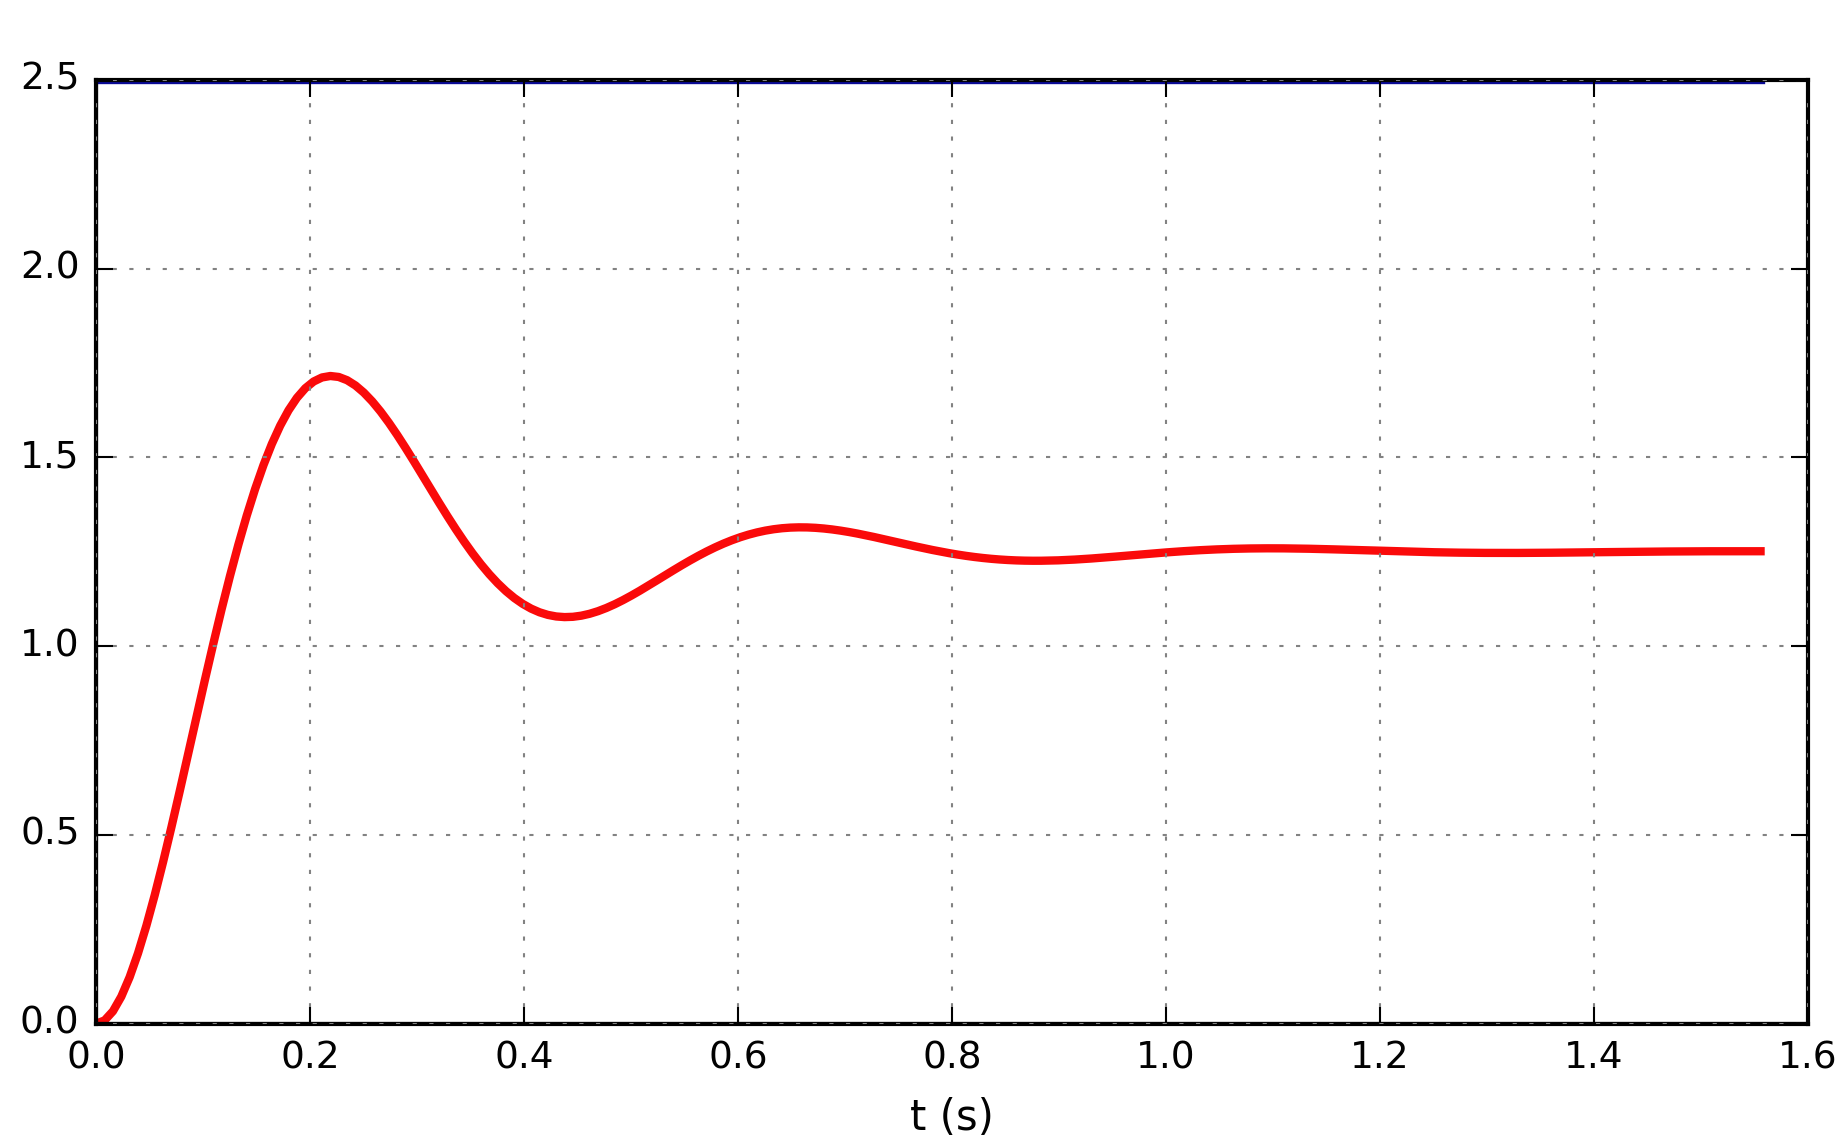
\includegraphics[width=\linewidth]{fig_02}
\end{center}

On considère dans un premier temps le système sans correction : $C(p)=1$.

\subparagraph{}\textit{Déterminer la fonction de transfert de la boucle interne $H_{\text{PM I}}(p) = \dfrac{X(p)}{\varepsilon(p)}$, en fonction de $K_e$, $K_0$, $m$, $K_P$ et $K_D$. Préciser les conditions
sur $K_D$ et $K_P$ pour que $H_{\text{PM I}}(p)$ soit stable en boucle ouverte}
\ifprof
\begin{corrige}
Même si la question n'est pas explicite, il s'agit de déterminer la FTBO. 

$H_{PMI}(p)=\dfrac{2K_0\left(K_P- K_e\right)}{mp^2+2K_0K_D+2K_0\left(K_P- K_e\right)}$. Le système est stable si 
$K_P> K_e$ et $K_D>0$.

\end{corrige}
\else
\fi

\subparagraph{}\textit{En considérant l’ensemble de l’asservissement, déterminer la
fonction de transfert $H_{\text{pert}}(p) = \dfrac{X(p)}{F_{\text{pert}}(p)}$, puis calculer les valeurs de $K_D$ et $K_P$
permettant de respecter les spécifications du cahier des charges en terme de
bande passante et d’amortissement (vous pourrez utiliser pour cette question l’abaque suivant).}
\ifprof
\begin{corrige}~\\

$H_{\text{pert}}(p) = \dfrac{X(p)}{F_{\text{pert}}(p)} = \dfrac{\dfrac{1}{2K_0\left(K_P- K_e\right)}}{1+\dfrac{K_D}{2\left(K_P- K_e\right)}p+\dfrac{mp^2}{4K_0\left(K_P- K_e\right)}}$.

On a $K=\dfrac{1}{2K_0\left(K_P- K_e\right)}$, $\omega_0 = \sqrt{\dfrac{4K_0\left(K_P- K_e\right)}{m}}$, $\xi = \sqrt{\dfrac{K_0K_D^2}{4m\left(K_P - K_e\right)}}$. 

Pour $\xi=0,4$, $\dfrac{\omega_{\SI{-3}{dB}}}{\omega_0}=1,2$. Cdc impose $\omega_{\SI{-3}{dB}}=\dfrac{\omega_{\text{max}}}{10}=\SI{314}{rad.s^{-1}}$ soit $\omega_0 =\dfrac{314}{1,2}=\SI{262}{rad.s^{-1}}$ $K_p = 5900$ et $K_D = 5,5$.
\end{corrige}
\else
\fi

\begin{center}
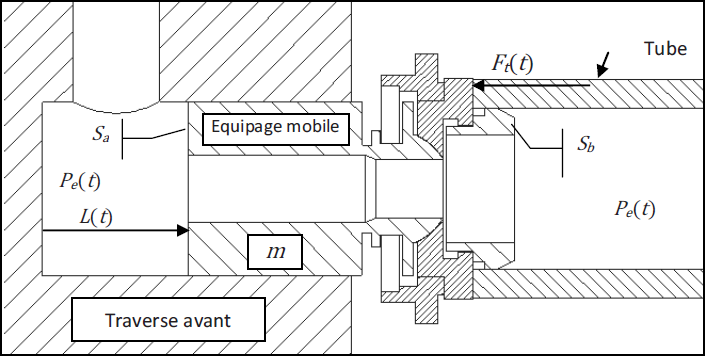
\includegraphics[width=\linewidth]{fig_03}
\end{center}


\subparagraph{}\textit{Tracer l'allure des diagrammes de Bode asymptotique et réel de la fonction
de transfert de la boucle interne $H_{\text{PM I}}(p)$ et préciser la pulsation de coupure ainsi que les marges de gain et de phase. Valider les critères de stabilité du cahier des charges.}
\ifprof
\begin{corrige}

\end{corrige}
\else
\fi

%L'ouverture et la fermeture des arrivées de gaz sont assurées par des « vannes
%guillotines ». À la suite de la fermeture de la guillotine, 
Le palier est soumis à un effort bref mais violent, qui peut être modélisé par une perturbation d'effort en
échelon d'amplitude $F_G$.

\subparagraph{}\textit{Conclure quant au critère de sensibilité vis-à-vis des perturbations.}
\ifprof
\begin{corrige}

\end{corrige}
\else
\fi

Afin d'améliorer les performances du système, on utilise un correcteur de fonction
de transfert : $C(p)=K_i\left(1+\dfrac{1}{T_i p} \right)$.

\subparagraph{}\textit{Quelle performance est directement améliorée par ce correcteur ? (justifier
votre réponse sans calcul).}
\ifprof
\begin{corrige}

\end{corrige}
\else
\fi

\subparagraph{}\textit{Tracer l'allure du diagramme de Bode du correcteur en précisant les
valeurs caractéristiques. Expliquer comment choisir $K_i$ et $T_i$ afin de conserver
des marges de gain, de phase, et une pulsation de coupure proches de celles obtenues
sans correction ($C(p)=1$). Proposer des valeurs numériques.}
\ifprof
\begin{corrige}

\end{corrige}
\else
\fi

On admet que le correcteur influe peu sur le temps de réponse et les dépassements
lorsque les marges de stabilité et la pulsation de coupure sont conservées.
On garde par conséquent les valeurs de $K_P$ et $K_D$ obtenues précédemment.

Conclusion : nous avons donc désormais dimensionné les deux boucles d'asservissement
successives permettant d'obtenir les performances attendues du palier
magnétique.

%Afin de préparer la prochaine partie, relative à l'étude dynamique du rotor, 
On recherche un modèle simple de l'effort du palier magnétique actif en fonction du
déplacement de l'arbre, dans une gamme de vitesses de rotation raisonnables
variant de $\SI{10000}{tr.min{-1}}$ à $\SI{30000}{tr.min{-1}}$.

\subparagraph{}\textit{Déterminer la fonction de transfert $K(p)$ telle que $F_T(p)=K(p)X(p)$.
À partir de simplifications justifiées, montrer que dans la plage de fréquences
considérée, l'effort $F_T(t)$ peut s'écrire sous la forme d'un modèle ressort amortisseur
$F_T(t)=-kx(t)-c\dot{x}(t)$ où vous préciserez les valeurs numériques de $k$ et $c$. Comment évolue le modèle lorsque
$\omega$ augmente au delà de cette plage de fréquences ?}
\ifprof
\begin{corrige}

\end{corrige}
\else
\fi


